\documentclass[12pt]{article}

\usepackage{amsmath,amsthm,amsfonts,amssymb,amsxtra}
\usepackage{pgf,tikz}
\usetikzlibrary{arrows}
\renewcommand{\theenumi}{(\alph{enumi})} 
\renewcommand{\labelenumi}{\theenumi}

\pagestyle{empty}
\setlength{\textwidth}{7in}
\setlength{\oddsidemargin}{-0.5in}
\setlength{\topmargin}{-1.0in}
\setlength{\textheight}{9.5in}

\newtheorem{problem}{Problem}

\begin{document}

\noindent{\large\bf MATH 242}\hfill{\large\bf Final Exam.}\hfill{\large\bf
  Spring 2012}\hfill{\large\bf Page 1/12}\hrule

\bigskip
\begin{center}
  \begin{tabular}{|ll|}
    \hline & \cr
    {\bf Name: } & \makebox[12cm]{\hrulefill}\cr & \cr
    {\bf 4-digit code:} & \makebox[12cm]{\hrulefill}\cr & \cr
    \hline
  \end{tabular}
\end{center}
\begin{itemize}
\item Write your name and the last 4 digits of your SSN in the space provided
above.
\item The test has twelve (12) pages, including this one, a table of Laplace
transforms (page \pageref{laplace}), and scratch paper (page
\pageref{scratch}).
\item The test is divided in two sections:  The first section (pages 2--4)
contains all the problems from the four different parts in which this course is
divided.  The second section (pages 6--11) contains blank paper where you will
work on the problems of your choice.  Start each problem by indicating clearly
the problem number, and the part it belongs to (e.g. \textit{Problem 6, Part
I})
\item Show sufficient work to justify all answers unless otherwise
  stated in the problem.  Correct answers with inconsistent work may
  not be given credit. 
\item Credit for each problem is given at the right of each problem
  number. 
\item No books, notes or calculators may be used on this test.
\end{itemize}
\hrule

\begin{center}
  \begin{tabular}{|c|c|c|}
    \hline
    &&\cr
    {\large\bf Part} & {\large\bf Max} & {\large\bf Points} \cr
    &&\cr
    \hline
    &&\cr
    {\Large I} & \Large 25 & \cr
    &&\cr
    \hline
    &&\cr
    {\Large II} & \Large 25 & \cr
    &&\cr
    \hline
    &&\cr
    {\Large III} & \Large 25 & \cr
    &&\cr
    \hline
    &&\cr
    {\Large IV} & \Large 25 & \cr
    &&\cr
    \hline\hline
    &&\cr
    {\large\bf Total} & \Large 100 & \cr
    &&\cr
    \hline
  \end{tabular}
\end{center}
\newpage

%%%%%%%%%%%%%%%%%%%%%%%%%%%%%%%%%%%%% Page 2

\noindent{\large\bf MATH 242}\hfill{\large\bf Final Exam.}\hfill{\large\bf
  Spring 2012}\hfill{\large\bf Page 2/12}\hrule

\vspace{0.5cm}
\noindent{\Large Part I.} Choose exactly three (3) problems from the list below that add up to 25 points.   Do each problem on a different half page.

{\problem[5pts] Find the general solution of the equation $3e^x \tan y +
(2-e^x) \sec^2 y \, \frac{dy}{dx} = 0$.}
{\problem[5pts] Find the particular solution of the equation $(1+e^x)yy'=e^x$
that satisfies the initial condition $y(0)=1$.}
{\problem[5pts] Find the equation of a curve that goes through the point
$(0,-2)$ and satisfies that the slope at any of its points is equal to three
plus the $y$--coordinate at that point.}
{\problem[10pts] Find the general solution of the equation $xy'=\sqrt{x^2-y^2}+y$.}
{\problem[10pts] Find the general solution of the equation $(x+y-2) + (x-y+4)y'=0$.}
{\problem[10pts] Find the general solution of the equation $y'+2xy=2xe^{-x^2}$}
{\problem[10pts] Find the general solution of the equation $xy'+y=y^2\ln x$.}
{\problem[10pts] Find the particular solution to the equation $y''=2y^3$ that satisfies the initial conditions $y(0)=1$ and $y'(0)=1$.}

\hrule

\vspace{0.5cm}
\noindent{\Large Part II.} Choose exactly three (3) problems from the list below that add up to 25 points.   Do each problem on a different half page.

{\problem[5pts] Plot a slope field for the differential equation
$x'=x^3(x^2-4)$, and use it to indicate the stability or instability of their
equilibria.}
{\problem[5pts] The time rate of change of an alligator population $P$ in a
swamp is proportional to the square of $P$.  The swamp contained a dozen
alligators in 1988, two dozen in 1998.  When will there be four dozen
alligators in the swamp?  What happens thereafter?}
{\problem[10pts] Suppose that the fish population $P(t)$ in a lake is attacked
by a disease at time $t=0$, with the result that the fish cease to reproduce
and the death rate is thereafter proportional to $1/\sqrt{P}$.  If there were
initially 900 fish in the lake, and 441 were left after 6 weeks, how long did
it take all the fish in the lake to die?}
{\problem[10pts] Consider an animal population $P(t)$ with constant death rate
$\delta = 0.01$ (deaths per animal per month) and with birth rate $\beta$
proportional to $P$.  Suppose that $P(0)=200$ and $P'(0)=2$.  When is $P=1000$?
When does doomsday occur?}
{\problem[5pts] The skid marks made by an automobile indicated that its brakes
were fully applied for a distance of $75\, m$ before it came to a stop.  The car
in question is known to have a constant deceleration of $20\, m/s^2$ under these conditions.  How fast (in $km/h$) was the car traveling when the brakes were first applied?}
{\problem[5pts] Find a general solution to the system}
\begin{equation*}
\begin{cases} 0 &=x' -4x+3y \\ 0&=-6x+y'+7y  \end{cases}
\end{equation*}
{\problem[10pts] Apply the Improved Euler method to solving numerically the
differential equation $y'=y-x-1$ with initial condition $y(0)=1$ in the
interval $[0,0.5]$.  Use a time-step $h=0.1$.  Prepare a table showing
four-decimal-place values of the approximate solution and the actual solution
at the points $x=0.1, x=0.2, x=0.3, x=0.4$ and $x=0.5$.}
\newpage

%%%%%%%%%%%%%%%%%%%%%%%%%%%%%%%%%%%%% Page 3

\noindent{\large\bf MATH 242}\hfill{\large\bf Final Exam.}\hfill{\large\bf
  Spring 2012}\hfill{\large\bf Page 3/12}\hrule

\vspace{0.5cm}
\noindent{\Large Part III.} Choose exactly three (3) problems that add up to 25 points from the list below.   Do each problem on a different half page.

{\problem[5pts] Find a function $y(x)$ such that $y^{(4)}(x)=y^{(3)}(x)$ for
all $x$, and $y(0)=18, y'(0)=12, y''(0)=13$, and $y^{(3)}(0)=7$.}
{\problem[10pts] Find a particular solution of the equation $2y''+4y'+7y=x^2$ using either the method of variation of parameters, or undetermined coefficients}.
{\problem[10pts] Use techniques based on Laplace transform to find the solution
of the initial value problem $y^{(4)}+2y''+y=4xe^x$ that satisfies the initial
conditions $y(0)=y'(0)=y''(0)=y^{(3)}(0)=0$.}
{\problem[5pts] Find the inverse Laplace transform of the function $F(s) =
\dfrac{s^2+1}{s^3-2s^2-8s}$.}
{\problem[10pts] Find the Laplace transform of the functions $f(x)=\dfrac{\sin
x}{x}$ and $g(x) = xe^{2x}\cos 3x$.}
{\problem[5pts] Show that $y_1=x^3$ and $y_2=\lvert x_3 \rvert$ are linearly
independent solutions on the real line of the equation $xy''-3xy'+3y=0$.
Verify that the Wronskian $W(y_1,y_2)$ is identically zero.  Why isn't this a
contradiction?}
\newpage

%%%%%%%%%%%%%%%%%%%%%%%%%%%%%%%%%%%%% Page 4
\noindent{\large\bf MATH 242}\hfill{\large\bf Final Exam.}\hfill{\large\bf
  Spring 2012}\hfill{\large\bf Page 4/12}\hrule

\vspace{0.5cm}
\noindent{\Large Part IV.} If you have received credit from your research
project, work only as many problems as you need to reach the 25 point threshold
(e.g. \textit{if you received 20 credit points, you only need to work a 5-point
problem in this part}).  Otherwise, choose exactly three (3) problems from the
list below that add up to 25 points.   Do each problem on a different half
page.


{\problem[5pts] A body of mass $m=0.5\, kg$ is attached to the end of a spring
that is stretched $2\, m$ by a force of $100\, N$.  It is set in motion with
initial position $x_0=1\, m$ and initial velocity $v_0=-5\, m/s$.  Find the
position of the body as well as the amplitude, frequency, period of oscillation
and time lag of its motion.}
{\problem[5pts] Interpret the following system as describing the interaction of two species with populations $x$ abd $y$.  Draw a slope field, and find the critical points.}
\begin{equation*}
\begin{cases} x' &= x(1.5-x-0.5y) \\ y' &= y(2-y-0.75x) \end{cases}
\end{equation*}
{\problem[5pts] A spherical tank of radius $4\, ft$ is full of gasoline when a circular bottom hole with radius $1\, in.$ is opened.  How long will be required for all the gasoline to drain from the tank?}
{\problem[10pts]\label{p:tanks} Consider two brine tanks connected as shown below.  Tank 1
contains $x(t)$ pounds of salt in $100\, gal$ of brine and tank 2 contains
$y(t)$ pounds of salt in $200\, gal$ of brine.  The brine in each tank is kept
uniform by stirring, and brine is pumped from each tank to the other at the
rates indicated.  In addition, fresh water flows into tank 1 at $20\, gal/min$,
and the brine in tank 2 flows out at $20\, gal/min$ (so the total volume of
brine in the two tanks remain constant).  The salt concentrations in the two
tanks are $x/100$ pounds per gallon, and $y/200$ pounds per gallon,
respectively.  Find a system of differential equations that model the rates of
change of the amount of salt in the two tanks, and solve it.}
{\problem[10pts]\label{p:circuit} For the circuit below, suppose that $L= 5\, H$, $R = 25\, \Omega$, and the source $E$ of emf is a battery supplying $100\, V$ to the circuit.  Suppose also that the switch has been in position 1 for a long time, so that a steady current of $4 A$ is flowing in the circuit.  At time $t=0$ the switch is thrown to position 2, so that $I(0)=4$ and $E=0$ for $t \geq 0$.  Find $I(t)$.}

\begin{center}
\begin{tabular}{cc}
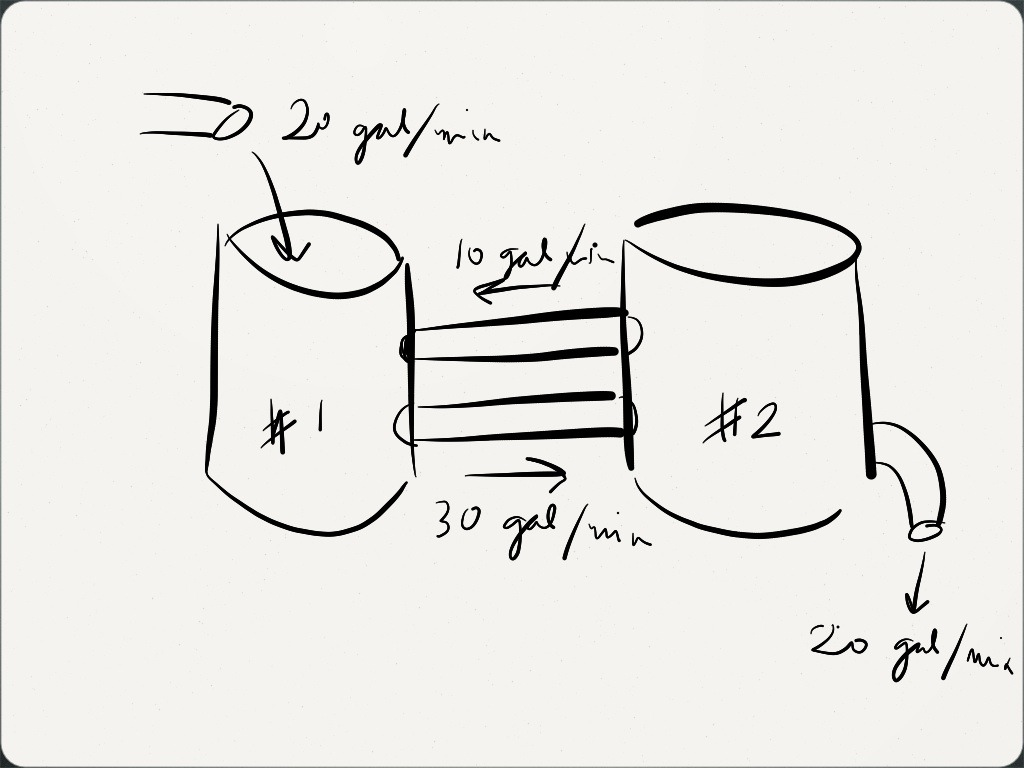
\includegraphics[width=0.4\linewidth]{tanks} &
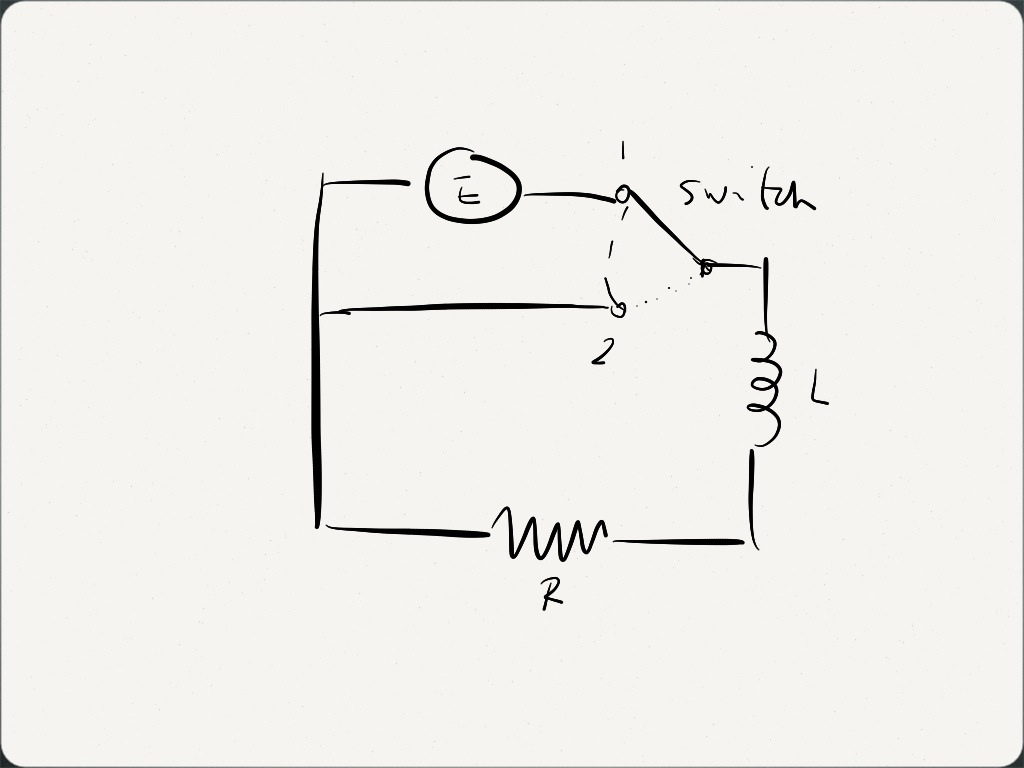
\includegraphics[width=0.4\linewidth]{circuit} \\
Figure for problem \ref{p:tanks} & Figure for problem \ref{p:circuit}
\end{tabular}
\end{center}
\newpage

%%%%%%%%%%%%%%%%%%%%%%%%%%%%%%%%%%%%% Page 5
\noindent{\large\bf MATH 242}\hfill{\large\bf Final Exam.}\hfill{\large\bf
  Spring 2012}\hfill{\large\bf Page 5/12}\hrule

\bigskip
\begin{center}\label{laplace}
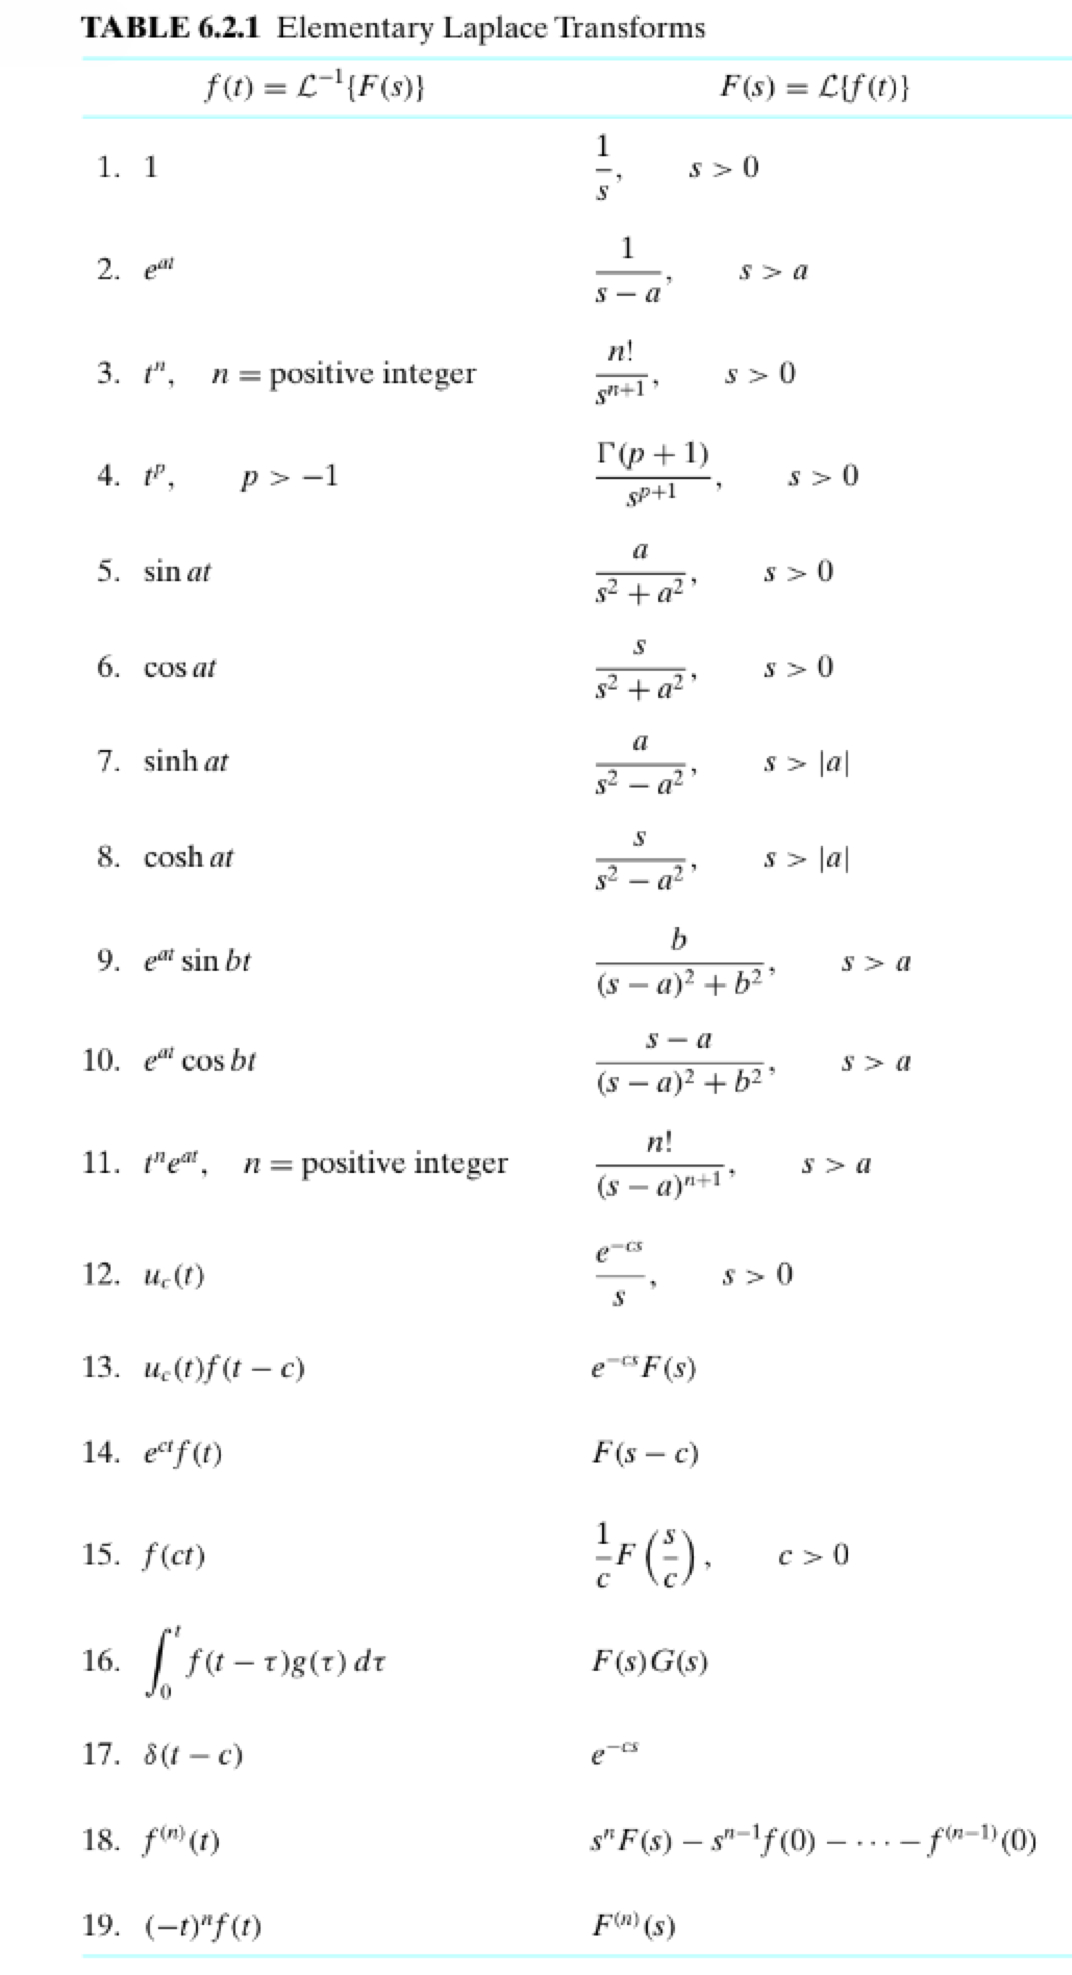
\includegraphics[width=0.7\linewidth]{table}
\end{center}


%%%%%%%%%%%%%%%%%%%%%%%%%%%%%%%%%%%%% Page 6
\noindent{\large\bf MATH 242}\hfill{\large\bf Final Exam.}\hfill{\large\bf
  Spring 2012}\hfill{\large\bf Page 6/12}\hrule

\vspace{13cm}
\hrule
\newpage

%%%%%%%%%%%%%%%%%%%%%%%%%%%%%%%%%%%%% Page 7
\noindent{\large\bf MATH 242}\hfill{\large\bf Final Exam.}\hfill{\large\bf
  Spring 2012}\hfill{\large\bf Page 7/12}\hrule

\vspace{13cm}
\hrule
\newpage
%%%%%%%%%%%%%%%%%%%%%%%%%%%%%%%%%%%%% Page 8
\noindent{\large\bf MATH 242}\hfill{\large\bf Final Exam.}\hfill{\large\bf
  Spring 2012}\hfill{\large\bf Page 8/12}\hrule

\vspace{13cm}
\hrule
\newpage
%%%%%%%%%%%%%%%%%%%%%%%%%%%%%%%%%%%%% Page 9
\noindent{\large\bf MATH 242}\hfill{\large\bf Final Exam.}\hfill{\large\bf
  Spring 2012}\hfill{\large\bf Page 9/12}\hrule

\vspace{13cm}
\hrule
\newpage
%%%%%%%%%%%%%%%%%%%%%%%%%%%%%%%%%%%%% Page 10
\noindent{\large\bf MATH 242}\hfill{\large\bf Final Exam.}\hfill{\large\bf
  Spring 2012}\hfill{\large\bf Page 10/12}\hrule

\vspace{13cm}
\hrule
\newpage
%%%%%%%%%%%%%%%%%%%%%%%%%%%%%%%%%%%%% Page 11
\noindent{\large\bf MATH 242}\hfill{\large\bf Final Exam.}\hfill{\large\bf
  Spring 2012}\hfill{\large\bf Page 11/12}\hrule

\vspace{13cm}
\hrule
\newpage
%%%%%%%%%%%%%%%%%%%%%%%%%%%%%%%%%%%%% Page 12
\noindent{\large\bf MATH 242}\hfill{\large\bf Final Exam.}\hfill{\large\bf
  Spring 2012}\hfill{\large\bf Page 12/12}\hrule

\vspace{0.5cm}
\large{Extra Scratch paper}\label{scratch}
\end{document}
